%
% main.tex -- Paper zum Thema wwt
%
% (c) 2019 Michael Schmid, Hochschule Rapperswil
%
\chapter{Wetter-Wavelet-Transformation\label{chapter:wwt}}
\lhead{Wetter-Wavelet-Transformation}
\begin{refsection}
\chapterauthor{Michael Schmid}



\definecolor{codegreen}{rgb}{0,0.6,0}
\definecolor{codegray}{rgb}{0.5,0.5,0.5}
\definecolor{codepurple}{rgb}{0.58,0,0.82}
\definecolor{backcolour}{rgb}{0.95,0.95,0.92}

\lstdefinestyle{mystyle}{
	backgroundcolor=\color{backcolour},   
	commentstyle=\color{codegreen},
	keywordstyle=\color{magenta},
	numberstyle=\tiny\color{codegray},
	stringstyle=\color{codepurple},
	basicstyle=\footnotesize,
	breakatwhitespace=false,         
	breaklines=true,                 
	captionpos=b,                    
	keepspaces=true,                 
	numbers=left,                    
	numbersep=2pt,                  
	showspaces=false,                
	showstringspaces=false,
	showtabs=false,                  
	tabsize=2
}
\lstset{style=mystyle}
\lstdefinestyle{mystyle}{
	morekeywords={cwt,contourf,datetick}
}


\section{Einführung}
\rhead{Einführung}


Seit Langem konsultiere ich meine aktuellen Wetterdaten über eine eher unübliche Internetseite.
Dabei handelt es sich um eine privat geführte Wetterstation, welche die gemessenen Daten im Internet grafisch darstellt.
Die Daten werden auch tabellarisch zur Verfügung gestellt.
Das Feature, welches ich bis anhin am regelmässigsten nutzte, war die grafische Darstellung der aktuellen Wetterdaten über den Zeitraum der letzten 24 Stunden.
Bei speziellen Ereignissen im Wetterverlauf fielen mir besondere und wiederkehrende Charakteristiken auf.
\\

Nach der Einführung in die Theorie der Wavelets kam mir die Idee, solche Wetterphänomene mit einer geeigneten Wavelet Transformation zu detektieren.
In diesem Paper wird einerseits auf die theoretischen Grundlagen der angewandten Methoden zurückgegriffen sowie die besprochenen meteorologischen Phänomene kurz erläutert. 
Weiterführend wird auf die verwendeten Methoden, auch in der praktischen Anwendung, vertieft eingegangen.
Ein besonderes Augenmerk wird auf die allgemeine Vorgehensweise sowie deren Schwierigkeiten gelegt.
\\




\section{Wetterstation Seegräben}
\rhead{Wetterstation Seegräben}

Die angesprochene Wetterstation in der Gemeinde Seegräben im Kanton Zürich ist mit einer DAVIS Vantage Pro2 6153 \cite{online:davisinstruments} realisiert worden.
Sie verfügt über Sensoren für die Temperatur, Feuchtigkeit, Geschwindigkeit und Richtung des Windes sowie für den Niederschlag. 
Durch diese Sensoren werden folgende Daten aufgezeichnet:


\begin{itemize}
	\item \textbf{Aussentemperatur} in Grad Celsius
	\item \textbf{Relative Luftfeuchtigkeit} in Prozent
	\item \textbf{Luftdruck} in hPa
	\item \textbf{Windgeschwindigkeit} in km/h, gemittelt über 5 Minuten
	\item \textbf{Windböen} in km/h
	\item \textbf{Windrichtung} nach Himmelsrichtung
	\item \textbf{Regenmenge} in $\text{l/m}^{2}$
\end{itemize}	


Der Thermo- / Feuchtigkeitssensor liegt zusammen mit dem Regenmengenmesser auf 2 Meter über Boden.
Mit einem Abstand von rund 10 Meter zum nächsten Gebäude sind optimale Messbedingungen geschaffen.
Mit einem Mast ist der Windmesser auf 1.5 Meter über dem First eines Gebäudes lokalisiert \space \cite{online:wss}.
Die Daten werden anschliessend mit einer Software von PC-Wetterstation.de weiterverarbeitet und auf der Website \cite{online:wss} veröffentlicht.
Mehr zur Verwendung der Wetterdaten im n\"achsten Abschnitt.

\section{Datenaufarbeitung}
\rhead{Datenaufarbeitung}
Der n\"achste Vorbereitungsschritt zur Wavelet Transformation war die Aufbereitung der zur Verf\"ugung gestellten Daten der Wetterstation. Dazu musste erst analysiert werden, wie die Daten auf der Website dargestellt werden.
\subsection{Wetter-Archiv}
Auf der Website gibt es mehrere Möglichkeiten, sich Wetterdaten aus der Vergangenheit darstellen zu lassen.
In der Kategorie des Archivs auf der Website kann man die Wetterdaten eines gew\"unschten Zeitraums tabellarisch oder grafisch darstellen lassen.
Vom Betreiber der Website steht keine Funktion zur Verfügung, welche es erlaubt, die Daten offiziell und automatisch herunterzuladen.
\subsection{Datenerfassung}
Da f\"ur die angestrebte Anwendung eine m\"oglichst hohe Aufl\"osung der jeweiligen Daten erforderlich ist, mussten die Daten im Zeitraum von einem Tag dargestellt werden.
Dies hatte zur Folge, dass man f\"ur jeden Tag eine Tabelle auf dem Archiv der Website \"offnen musste. Man hätte anschliessend die Daten mit \textit{copy and paste} in eine Excel-Tabelle einf\"ugen können. Daher wurde  entschieden, ein Programm zu schreiben, welches diese Aufgabe automatisieren sollte.
Als Programmiersprache wurde hierf\"ur Python gewählt.


Mit der \textit{Pandas Library} und der Funktion \texttt{'read\_html'} \space konnten die Daten direkt aus dem Python Programm von der Website heruntergeladen werden.
Entscheidend für das Gelingen dieser Teilaufgabe war, dass die URL-Links der einzelnen Tage stets regelmässig aufgebaut sind:
\\
\\
$$\centering{\textit{https://www.wetter-seegraeben.ch/uploads/insert.php?insert=\textbf{20190701}.htm}}$$
\\
Wie zu sehen ist, wird der Link mit dem Datum regelmässig aufgebaut. Somit konnten die entsprechenden Links mit mehreren While-Schleife zusammengesetzt werden.
In der Abbildung \ref{fig:python-code} ist der wesentliche Ausschnitt aus dem Python Code dargestellt.
\begin{figure}
	\centering
	\lstinputlisting[language=Python,firstline=1,lastline=16,numbers=left,style = Python]{papers/wwt/code/get_data.py}
	\caption{Python Codeausschnitt}
	\label{fig:python-code}
\end{figure}
Die Daten konnten im nächsten Schritt in einer Excel-Tabelle abgespeichert werden.
Dort folgte der letzte Feinschliff; d.h. alle überflüssigen Kopfzeilen und Statistiken wurden entfernt.

\subsubsection{Unregelmässigkeiten der Wetterstation}
Bei der Datenerfassung durch das eben beschriebene Python Programm wurden einige Unregelmässigkeiten der Wetterstation beobachtet.
Das Programm wird jeweils durch eine Fehlermeldung abgebrochen, wenn der angegebene Link nicht abrufbar ist. 
So fiel auf, dass unregelmässig auf das Jahr verteilt, Daten von gewissen Tagen fehlten. Es stellte sich heraus, dass hinter dem eigentlich korrektem Link die entsprechende Internetseite nicht zur Verfügung steht.
Wird manuell auf der Website nach diesem Tag gesucht, kann nichts gefunden werden.
Dies trat teilweise sogar in Abschnitten von mehreren Tagen auf.
Wie sich später herausstellte, traten die fehlenden Tagen nicht zu den Zeitpunkten auf, die mich interessierten.


\subsection{Datendarstellung}
Die Darstellung der gewonnenen Daten konnte einfach mittels Python realisiert werden.
Anbei in Abbildung \ref{fig:rawdata} der Plot der Rohdaten aus dem Jahre 2018, wobei nur jeder zehnte Messpunkt verwendet wurde.
Diese Rohdaten dienten als Grundlage für alle weiteren Berechnungen. 
\begin{figure}
	\centering
	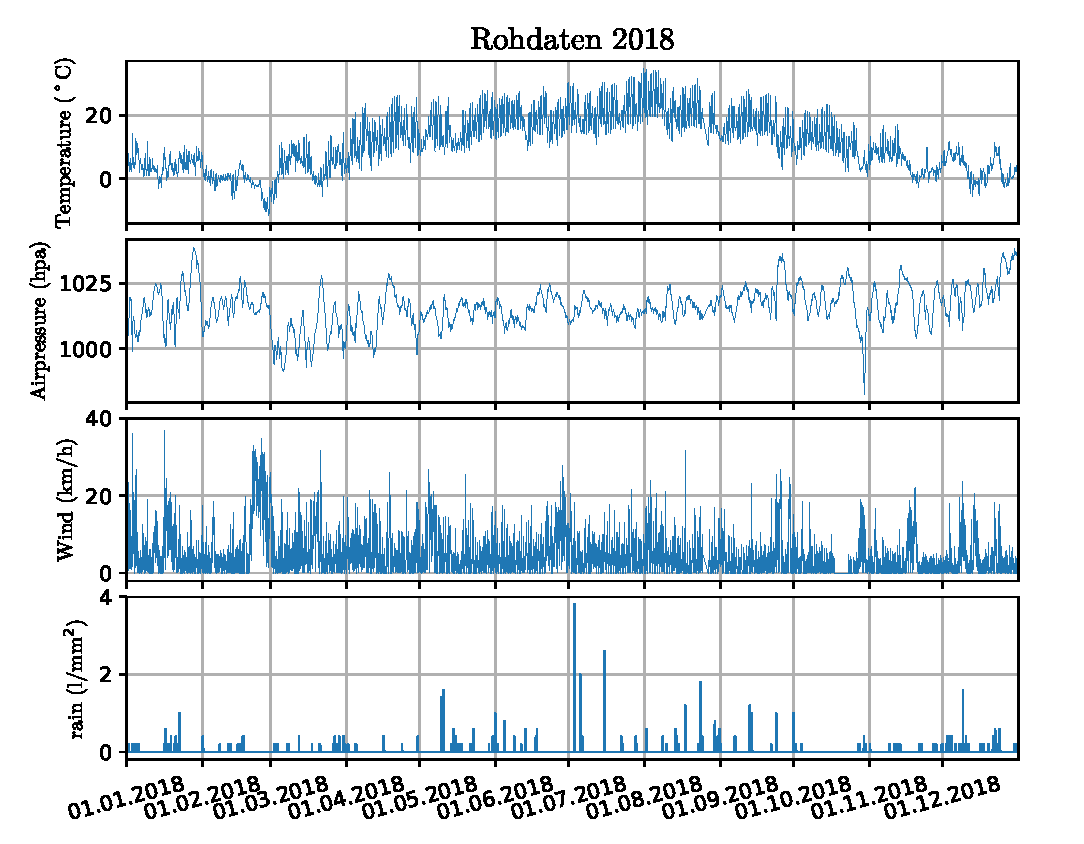
\includegraphics[width=1\textwidth]{papers/wwt/images/raw.pdf}
	\caption{Rohdaten 2018}
	\label{fig:rawdata}
\end{figure}


\section{Stetige Wavelet-Transformation}
\rhead{Stetige Wavelet-Transformation}
Die theoretischen Grundlagen rund um die stetige Wavelet-Transformation wurden im Kapitel \ref{chapter:cwt} genauestens erläutert. 
In diesem Abschnitt der Seminararbeit wird öfters auf die Theorie des angesprochenen Kapitels \ref{chapter:cwt} referenziert ohne diese genauer zu erläutern. 

Für eine m"oglichst aussagekräftige Untersuchung der Signale, in welcher so viele Informationen gewonnen werden sollten wie m"oglich, eignet sich die stetige Wavelet-Transformation (folgend noch kurz \textit{cwt} aus dem Englischen "continuous wavelet transform"). 
Regelmässig auftretende Frequenzen können dank der \textit{cwt} gefunden und zusätzlich einem Zeitraum zugeordnet werden.
\subsection{Das verwendete Wavelet}
In
\begin{equation}
\mathcal{W}f (a,b)
=
\langle f,\psi_{a,b}\rangle
=
\frac{1}{\sqrt{|a|}}\int_{-\infty}^\infty f(t)\,\overline{
	\psi\biggl(\frac{t-b}{a}\biggr)}\,dt
\label{eq:cwt1}
\end{equation}
erkennt man die grundlegende Formel der \textit{cwt}.
Wobei das $\psi_{a,b}$ für das Mutter-Wavelet steht, welches mit dem Koeffizienten $a$ skaliert und mit $b$ verschoben wird.

Als Mutter-Wavelet wurde 
\begin{equation}
\psi_{Gabor}(t) =  c_{\sigma} e^{-\frac{1}{2}t^2} \biggl(e^{i \sigma t}- e^{-\frac{1}{2} \sigma^2} \biggr)
\label{eq:morlet}
\end{equation} \cite{online:Morlet}
verwendet, welches auch als das analytische Gabor-Wavelet bekannt ist.
Dabei gibt $\sigma$ an, wie hoch die Frequenz ist und dementsprechend auch, wie viele lokale Maxima und Minima innerhalb des Gauss'schen Fensters das Mutter-Wavelet existieren.
Weiter ist $c_{\sigma}$ eine reelle Konstante und dient zur Erf"ullung der Zulässigkeitsbedingungen in der Definition \ref{cwt:zulaessig}.
Das Gabor-Wavelet wird in der Abbildung \ref{fig:gabor_plot} \space dargestellt und $\sigma$ wurde auf 5 gesetzt.

\begin{figure}[h]
\centering
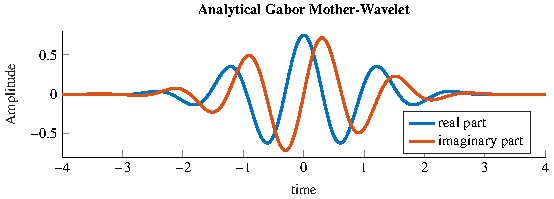
\includegraphics[width=1\textwidth]{papers/wwt/images/gabor.pdf}
\caption{Analytisches Gabor Mutter-Wavelet}
\label{fig:gabor_plot}
\end{figure}

Weiter ist zu erwähnen, dass das eben gezeigte Gabor Wavelet der referenzierten Quelle entnommen wurde. Ob Matlab die selbe Form verwendet, konnte nicht abschliessend geklärt werden.

\subsection{Berechung mit Matlab}
\label{matlab}
Die Berechnung der \textit{cwt} wurde mit der numerischen Berechnungs-Software Matlab durchgeführt.
Die dafür verwendete Funktion war die cwt()-Funktion.
Die Funktion arbeitete bei korrekter Parametrisierung wie gewünscht.
Falls man verstehen möchte wie die Funktion genau rechnet, muss man sich mit einer eher dürftigen Dokumentation herumschlagen.
Folgende Parameter wurden verwendet
\lstinputlisting[language=Matlab,firstline=1,lastline=1,  numbers=left, style = mystyle]{papers/wwt/code/matlab.m}
\label{fig:matlab_code_cwt}
wobei Matlab das Gabor-Wavelet als \texttt{'amor'} bezeichnet, mit \texttt{'VoicesPerOctave'} konnte die Genauigkeit erhöht werden und die Variable \texttt{'fs'} beschreibt die Abtastfrequenz der Messsignale.
Bei den Rückgabewerten werden die Wavelet-Werte in \texttt{'wt'} als komplexe Matrix und die approximierten Frequenzen in \texttt{'F'} abgespeichert.

\begin{figure}[h]
	\centering
	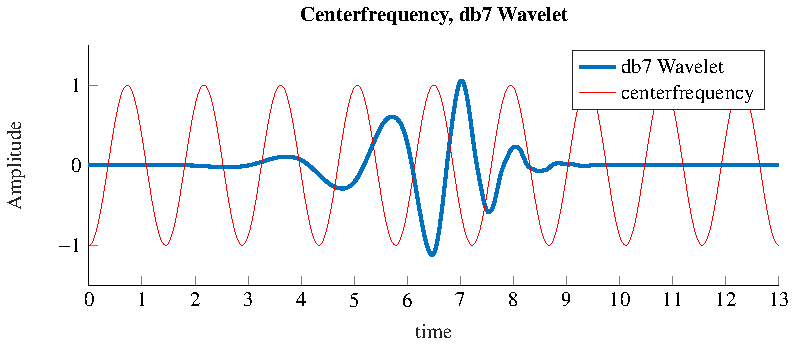
\includegraphics[width=1\textwidth]{papers/wwt/images/centerf.pdf}
	\caption{Approximierte Frequenz eines db7-Wavelet}
	\label{fig:centerf}
\end{figure}


Anstelle des Skalierungsfaktors $a$ in der Gleichung \eqref{eq:cwt} berechnet Matlab eine approximierte Frequenz und gibt diese zurück.
Für jeden verwendeten Skalierungsfaktor $a$ wird eine Sinuskurve gesucht, die am ehesten mit der Frequenz des entsprechenden Wavelets übereinstimmt.
Siehe das Beispiel mit einem Daubechies Wavelet der Nummer 7 in der Abbildung \ref{fig:centerf}.


Dies dient dazu den Wavelet-Koeffizienten einer Frequenz zuzuordnen. 
Aus dem verwendeten Skalierungsfaktor $a$ könnte auf die Schnelle keine Information entnommen werden.


\subsection{Verifikation der approximierten Frequenz}
\label{Freq}
Diese approximierte Frequenz konnte man mit den geeigneten Daten aus der aktuellen Anwendung der Wetterdaten sehr gut verifizieren.
Der Temperaturverlauf während einer Hochdruckphase ist sehr regelmässig und man sollte den 24 Stunden Tagesverlauf exakt erkennen.

Dank der Regelm"assigkeit des Temperaturverlaufs sieht man im \textit{cwt}-Plot eine Erh"ohung des Wertes bei einer gewissen Frequenz.
Die ausgelesene Frequenz beträgt $f = 1.16\cdot10^{-5} \,\text{Hz}$, die umgerechnet einer Periodendauer von $T = 86206.897\,\text{s}\approx 23\,\text{h }56\,\text{min } 47\,\text{s}$ entspricht.
Damit kann die Frequenz im Rückgabewert der Matlab-Funktion als sehr genau bezeichnet werden.
Dabei kommt weiter dazu, dass nur alle f"unf Minuten ein Datenpunkt aufgenommen wurde und somit die Abweichung zu 24 Stunden kleiner ist als die eigentliche Auflösung.

\begin{figure}[h]
	\centering
	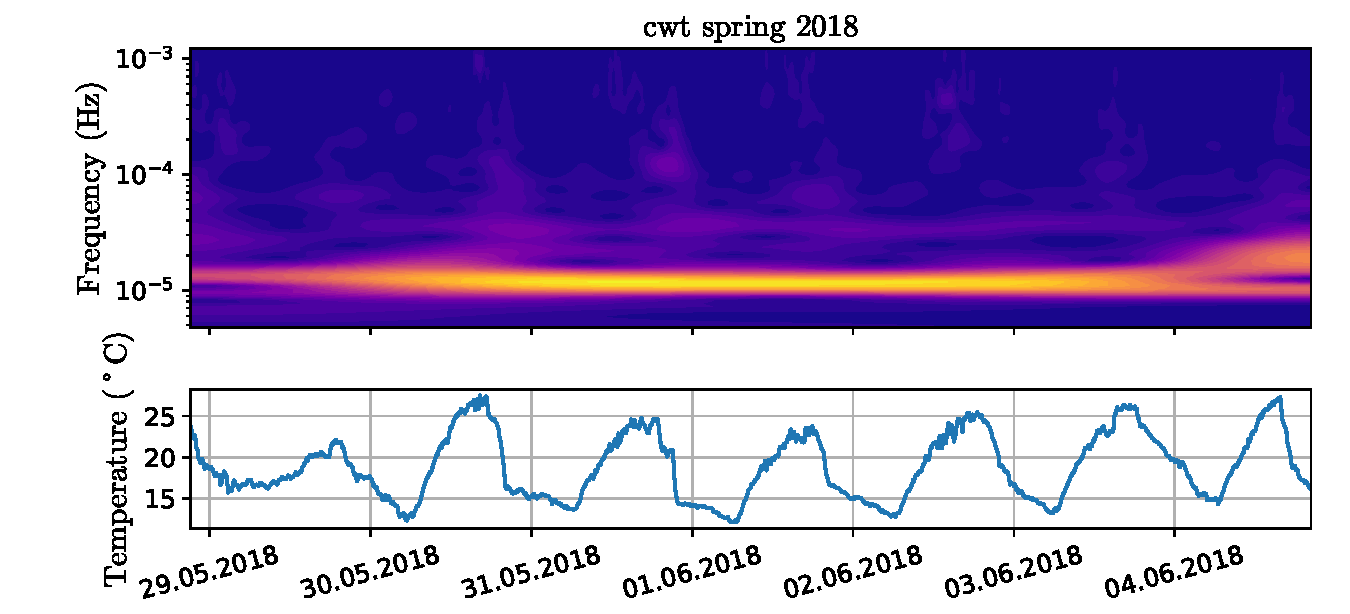
\includegraphics[width=1\textwidth]{papers/wwt/images/data_spring.pdf}
	\caption{Temperaturverlauf und entsprechende cwt}
	\label{fig:cwt_zoom}
\end{figure}



\section{Analyse von Wettereignissen}
\rhead{Analyse von Wetterereignissen}
Aufgrund der Kenntnisse rund um die \textit{cwt} kann angenommen werden, dass ein Wechsel in der Frequenz gut detektiert werden kann.
Bei einer typischen Sturmfront, welche öfters als Wintersturm in den Monaten Dezember und Januar auftreten, zeigten sich bei der Konsultation der Wetterdaten rapide Temperatur- und Luftdruckwechsel sowie ein erhöhtes Windaufkommen.
Das Ziel der Analyse war, solche Ereignisse mittels einer geeigneten \textit{cwt} zu detektieren.
Bei den Rohdaten der Frontdurchgängen erkennt man gemeinsame Wechsel im Wind, der Temperatur sowie dem Luftdruck, daher kann in der Wavelet-Transformation eine erkennbare Antwort erwartet werden. 
Diese korrelierenden auftretenden Frequenzen sollten in der \textit{cwt} sichtbar sein.

\subsection{Parallelen zur Kovarianz}
Um das korrelierende Auftreten der einzelnen Datenkanäle zu verdeutlichen, wurden bei diesen jeweils die zwei zusammengehörenden Resultate der \textit{cwt} miteinander multipliziert. 
Dabei werden die Stellen hervorgehoben, wo beispielsweise der Luftdruck und die Windgeschwindigkeit abhängig voneinander variieren. 
Sprich die Resultate der \textit{cwt} gemeinsam und zum selben Zeitpunkt für den Luftruck und Wind gross sind.
Dies funktioniert besonders gut, da die Werte rasch gegen null gehen, falls nur schon einer der beiden Datenverläufe nicht mit dem aktuellen Mutter-Wavelet übereinstimmt.


Genauer betrachtet zeigt das Verfahren mit der Multiplikation Ähnlichkeiten mit der Formel
\begin{equation}
COV(X,Y) = \frac{\sum_{i=1}^{N} (x_i- \bar{x})(y_i- \bar{y})}{N-1}
\label{eq:kovarianz}
\end{equation}
oder bei stetigen Werten
\begin{equation}
COV(X,Y) = \int_{-\infty}^\infty (x(t)- \bar{x})(y(t)- \bar{y}) \text{\space}dt
\label{eq:kovarianz_int}
\end{equation}
der Kovarianz aus der Statistik. 
Die Kovarianz zeigt sich nicht nur in dieser Anwendung. Auch schon bei der grundlegenden Formel \eqref{eq:cwt1} der \textit{cwt}, kann man gewisse Parallelen sehen. 
In \eqref{eq:cwt1} ist die Motivation, die jeweiligen Parameter $a$ und $b$ zu finden, bei welchen das Mutter-Wavelet und das Signal gemeinsam variieren.
Auch hierfür werden die Produkte der Signale berechnet, auf integriert und gemittelt.
Auch dies ist eine etwas abgewandelte Art der Kovarianz zwischen dem Datensignal und dem Mutter-Wavelet.

Setzt man den \textit{Luftdruck} und das Mutter-Wavelet $\psi_{a,b}$ in \eqref{eq:kovarianz_int} ein,

\begin{equation}
COV(\text{\textit{Luftdruck}}, \psi_{a,b}) = \int_{-\infty}^\infty (\text{\textit{Luftdruck}}(t)- \overline{\text{\textit{Luftdruck}}})(\psi_{a,b}(t)- \overline{\psi_{a,b}}) \text{\space}dt,
\end{equation}
kann wie folgt umgeformt werden.
Gemäss den Zulässigkeitsbedingungen eines Mutter-Wavelets ist $\overline{\psi_{a,b}} = 0$ (Definition \ref{cwt:zulaessig}). Weiter werden Multiplikationen in Skalarprodukte umgewandelt, somit folgt
\begin{equation}
COV(\text{\textit{Luftdruck}}, \psi_{a,b}) =  \int_{-\infty}^\infty\langle \text{\textit{Luftdruck}}(t)- \overline{\text{\textit{Luftdruck}}},\psi_{a,b}(t) \rangle \text{\space}dt.
\end{equation}
Weiter ausmultipliziert
\begin{equation}
COV(\text{\textit{Luftdruck}}, \psi_{a,b}) = \int_{-\infty}^\infty	\langle \text{\textit{Luftdruck}}(t),\psi_{a,b}(t)\rangle - \langle \overline{\text{\textit{Luftdruck}}},\psi_{a,b}(t)\rangle \text{\space}dt,
\end{equation}
schlussendlich ergibt sich mit $\langle \overline{\text{\textit{Luftdruck}}},\psi_{a,b}(t) \rangle = 0$,
\begin{equation}
\begin{split}
COV(\text{\textit{Luftdruck}}, \psi_{a,b}) &= \int_{-\infty}^\infty \langle \text{\textit{Luftdruck}}(t),\psi_{a,b}(t)\rangle \text{\space}dt \\
\label{eq:wwt_kovarianz}
\end{split}
\end{equation}

damit ist die Vereinfachung komplett.


\subsection{Multiplikation der Resultate zweier Wavelet-Transformationen}

Wie schon bei der Kovarianz gezeigt, wird bei der \textit{cwt} ein grosses Resultat des Produktes anzeigen, dass beide Datenkanäle mit der selben Frequenz auf ein gewisses $\psi_{a,b}$ ansprechen.  

Wobei zuerst separat die \textit{cwt}, 
\begin{equation}
\mathcal{W}\text{\textit{Luftdruck}}(a,b) = \langle \text{\textit{Luftdruck}},\psi_{a,b}\rangle
\end{equation}
\begin{equation}
\mathcal{W}\text{\textit{Wind}}(a,b) = \langle \text{\textit{Wind}},\psi_{a,b}\rangle,
\end{equation}
des Luftdruckes und des Windes berechnet wurde.
Als nächster Schritt wurde das Produkt der beiden Funktionen berechnet.

\begin{equation}
\mathcal{P}(\text{\textit{Luftdruck}},\text{\textit{Wind}})(a,b) = \mathcal{W}\text{\textit{Luftdruck}}(a,b) \cdot \mathcal{W}\text{\textit{Wind}}(a,b)
\label{eq:produkt-wwt}
\end{equation}

Ausgeschrieben auf die vollständige Formel der \textit{cwt} \eqref{eq:cwt1}

\begin{equation}
\begin{split}
\mathcal{P}(\text{\textit{Luftdruck}},\text{\textit{Wind}})(a,b)
& =
\langle \text{\textit{Luftdruck}},\psi_{a,b}\rangle \cdot \langle \text{\textit{Wind}},\psi_{a,b} \rangle \\
& = \frac{1}{\sqrt{|a|}}\int_{-\infty}^\infty \text{\textit{Luftdruck}}(t)\,\overline{
	\psi\biggl(\frac{t-b}{a}}\biggr)\,dt
\cdot
\frac{1}{\sqrt{|a|}}\int_{-\infty}^\infty Wind(t)\,\overline{
	\psi\biggl(\frac{t-b}{a}\biggr)}\,dt .
\label{eq:cwt_wwt}
\end{split}
\end{equation}

Die Formel \eqref{eq:wwt_kovarianz} kann, zum optimalen Vergleich mit \eqref{eq:cwt_wwt}, mit dem Produkt des Windes erweitert werden

\begin{equation}
\begin{split}
COV(\text{\textit{Luftdruck}}, \psi_{a,b})(a,b)\cdot COV(\text{\textit{Wind}}, \psi_{a,b})(a,b) \\ =  \int _{-\infty}^\infty \langle \text{\textit{Luftdruck}}(t),\psi_{a,b}(t)\rangle \text{\space}dt \cdot \int _{-\infty}^\infty \langle \text{\textit{Wind}}(t),\psi_{a,b}(t)\rangle \text{\space}dt,
\label{eq:cov_wwt}
\end{split}
\end{equation}

dabei kommt die Analogie, ohne die Korrekturfaktoren, zwischen den Formeln \eqref{eq:cov_wwt} und\eqref{eq:cwt_wwt} eindrücklich zur Geltung.

\subsubsection{Anwendung in Matlab}

Wie im Abschnitt \ref{matlab} beschrieben, berechnet Matlab mit der Funktion der \textit{cwt}, den Rückgabewert und gibt diesen als Matrix zurück.
Um \eqref{eq:produkt-wwt} anzuwenden werden die beiden gleichgrossen Matrizen des Resultates der \textit{cwt} miteinander elementweise,

\begin{equation}
	A\circ B=(a_{{ij}}\cdot b_{{ij}})={\begin{pmatrix}a_{{11}}\cdot b_{{11}}&\cdots &a_{{1n}}\cdot b_{{1n}}\\\vdots &\ddots &\vdots \\a_{{m1}}\cdot b_{{m1}}&\cdots &a_{{mn}}\cdot b_{{mn}}\end{pmatrix}},
\end{equation}
multipliziert \cite{online:schur}.




\subsection{Sturmsaison 2018}
\rhead{Sturmsaison 2018}
Bereits bekannt war, dass in der Sturmsaison im Jahre 2018 einige heftige Winterstürme aufgetreten sind.
So wurde bei der Analyse der Daten nur auf diese Periode das Augenmerk gelegt. 
In Abbildung \ref{fig:cwt_storm} \space sieht man die Wavelet-Transformation des Luftdruckes und Windes miteinander multipliziert.
Dies über die Monate Januar und Februar im Jahre 2018 hinweg.
Weiter wird der Luftdruck- und Windverlauf dargestellt.
 
\begin{figure}[h]
	\centering
	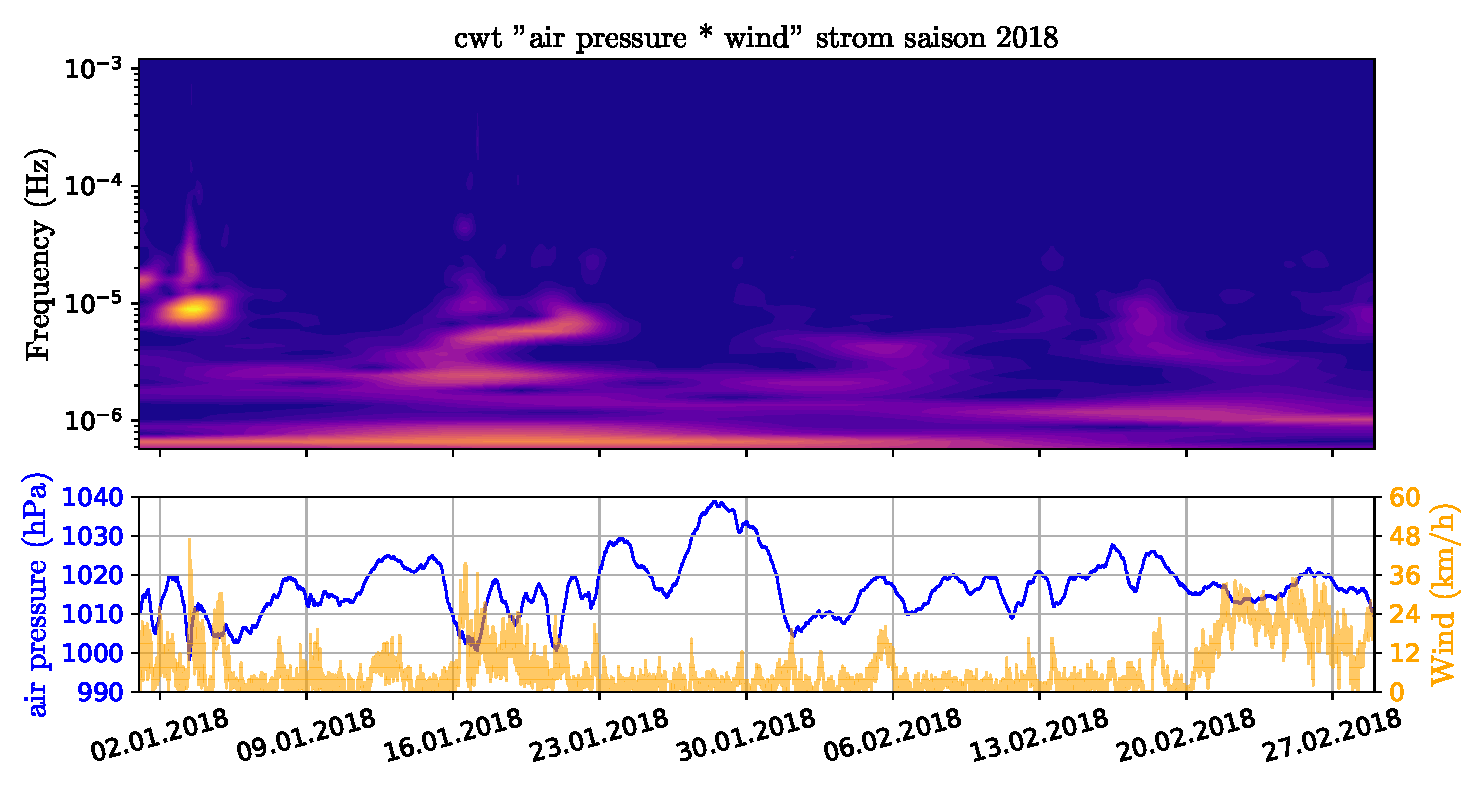
\includegraphics[width=1\textwidth]{papers/wwt/images/storm_airp_wind.pdf}
	\caption{Cwt und Rohdaten Sturmsaison 2018}
	\label{fig:cwt_storm}
\end{figure}

In Abbildung \ref{fig:cwt_storm} \space zeigen sich um den 3. sowie zwischen dem 16. und 23. Januar jeweils gewisse Frequenzen des Windes und des Luftdruckes, die gemeinsam auf die Wavelet-Transformation angesprochen haben.

\subsubsection{Wintersturm {\em Burglind} }
\label{burglind}
Hineingezoomt um den 3. Januar (Abbildung \ref{fig:cwt_storm_zoom}) sind im Rohdatenverlauf die Aktivitäten des Windes und Luftdruckes erkennbar. 
\begin{figure}[b]
	\centering
	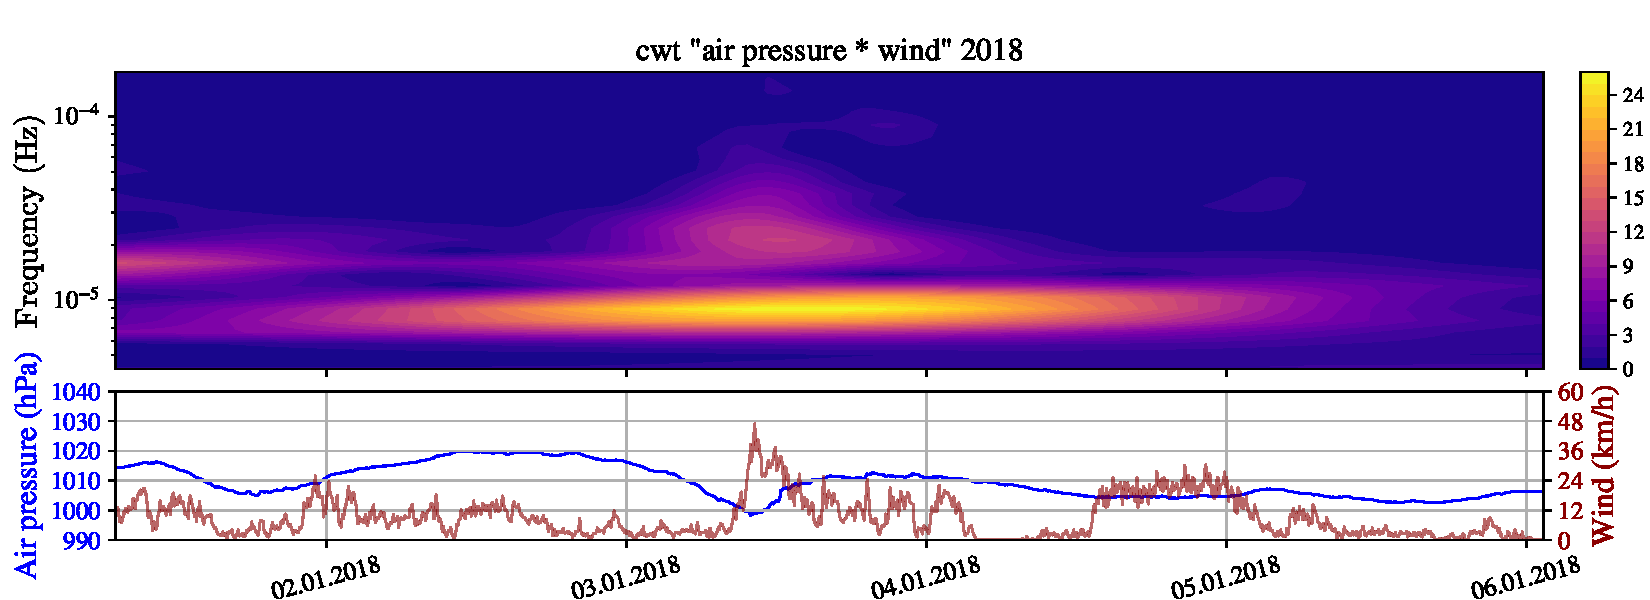
\includegraphics[width=1\textwidth]{papers/wwt/images/storm_airp_wind_zoom.pdf}
	\caption{Cwt und Rohdaten Wintersturm {\em Burglind}  2018}
	\label{fig:cwt_storm_zoom}
\end{figure}
Aus dem Fachbericht \space \cite{Fachbericht:Burglind} von MeteoSchweiz war bekannt, dass am Vormittag des 3. Januars 2018 die stärkste Sturmfront seit dem verheerenden Sturm Lothar aus dem Jahre 1999 über die Schweiz zog.
Dabei zeigt sich eindrücklich, wie der Sturmdurchgang in der multiplizierten Wavelet-Transformation hervorgehoben wird.

\subsubsection{Sturmtief {\em Evi}  und {\em Friederike} }
\label{evi}
Beim zweiten Ereignis zwischen dem 16. und 23. Januar trat die Aktivität nicht mehr so deutlich auf.
Nach dem Sturmarchiv  \cite{online:sturmarchiv} traf am 16. Januar das Sturmtief {\em Evi}  und am 18. Januar das Sturmtief {\em Friederike} auf Europa. Dabei zeigt sich nach der Amplitude, dass das Sturmtief nicht direkt auf die Schweiz traf, sonder diese lediglich streifte. 

\begin{figure}[h]
	\centering
	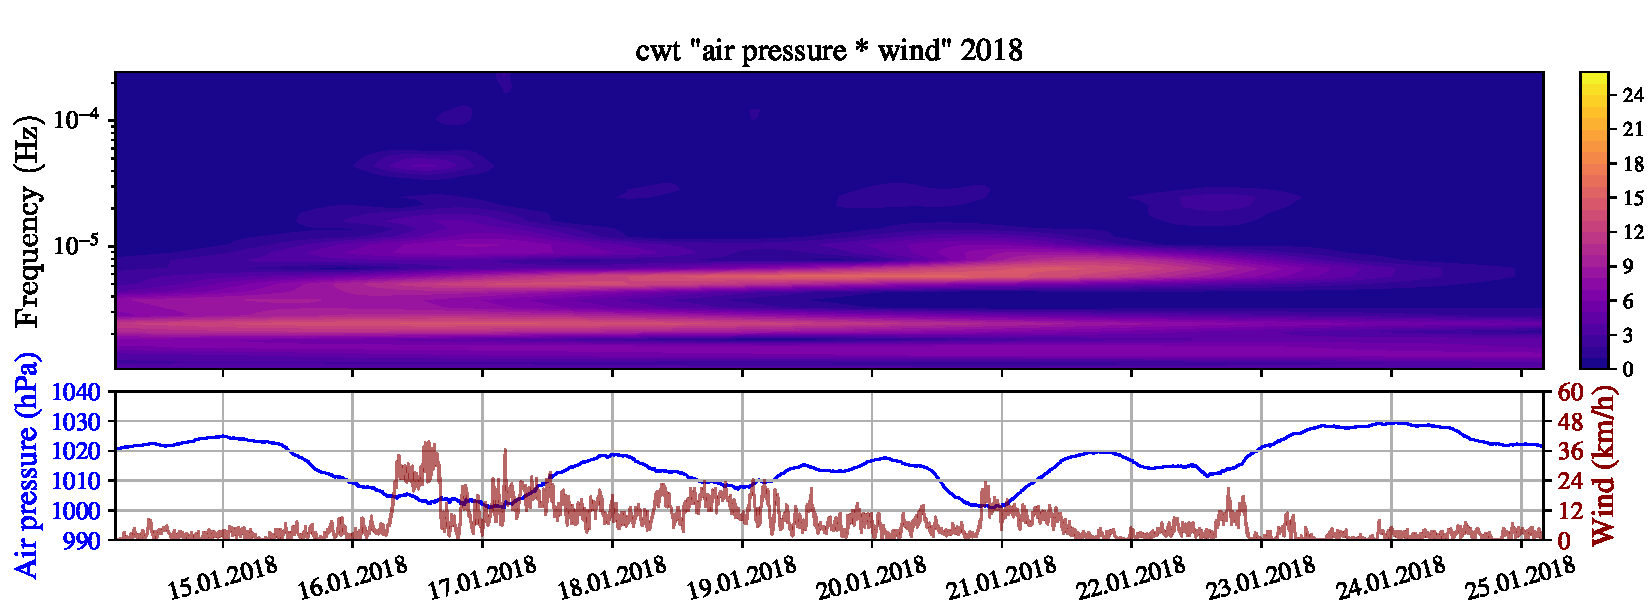
\includegraphics[width=1\textwidth]{papers/wwt/images/storm_airp_wind_zoom2.pdf}
	\caption{Cwt und Rohdaten Strumtief {\em Evi}  und {\em Friederike} 2018}
	\label{fig:cwt_storm_zoom2}
\end{figure}



\section{Schlussfolgerung}
\rhead{Schlussfolgerung}

Mit dem Versuch, die Wavelet-Transformation im Bereich der Wetteranalyse nützlich anzuwenden, zeigt sich, dass dies durchaus möglich ist.
In der Anwendung mit dem Phänomen der Winterstürme wurde die Wavelet-Transformation oder genauer die stetige Wavelet-Transformation erfolgreich eingesetzt.
Es können zwei Hypothesen aufgestellt werden:
\begin{itemize}
	\item Die periodischen Tagesverläufe bei konstanten Wetterverhältnissen führen dazu, dass die Wavelet-Koeffizienten der \textit{cwt} bei dieser Frequenz deutlich ansteigen (\ref{Freq}).
	
	\item Nicht periodische Ereignisse äussern sich durch das korrelierte Auftreten bei der Betrachtung mehrerer Datenkanäle. Dies kann mit dem Produkt der Wavelet-Koeffizienten oder eben der Kovarianz analysiert werden (\ref{burglind}).
\end{itemize}


Damit ist selbstverständlich noch nichts abschliessend bewiesen. Die Hypothesen müssten detaillierter analysiert werden.
Auch sollte die Methode weiterführend auf andere meteorologische Ereignisse angewandt werden.
Zum Beispiel könnte man versuchen, Gewitter zu detektieren.
Falls sich diese Methode für mehrere Phänomene beweisen lässt, ist eine praktische Anwendung möglich und durchaus vorstellbar. 

\section{Anhang}
Anbei in Abbildung \ref{fig:python-plot-code} und \ref{fig:python-plot-code2} der verwendete Code zum Plotten der Abbildung \ref{fig:cwt_storm}.

\begin{figure}[h]
	\centering
	\lstinputlisting[language=Python,firstline = 0, lastline = 39, numbers=left, firstnumber=0, style = Python]{papers/wwt/code/plot_burglind.py}
	\caption{Python Codeausschnitt}
	\label{fig:python-plot-code}
\end{figure}
\begin{figure}[h]
	\centering
	\lstinputlisting[language=Python,firstline = 40, lastline = 90, firstnumber=39, numbers=left,style = Python]{papers/wwt/code/plot_burglind.py}
	\caption{Python Codeausschnitt}
	\label{fig:python-plot-code2}
\end{figure}
 
 \newpage

\printbibliography[heading=subbibliography]
\end{refsection}
